\section{DenseNet}
\subsection{DenseNet là gì}
DenseNet - Dense Convolutional Network (Mạng Tích chập Kết nối Dày đặc) - là một trong những biến thể mở rộng của Resnet và là một kiến trúc mạng,trong đó mỗi lớp được kết nối trực tiếp với mỗi lớp khác nhau theo kiểu chuyển tiếp (trong mỗi khối dense block). Đối với mỗi lớp, các bản đồ đặc trưng (feature map) của tất cả các lớp ở phần trước được coi là các đầu vào riêng biệt và ở đó các bản đồ tính năng lại tiếp tục làm đầu vào cho tất cả các lớp tiếp theo. Cấu trúc mạng này mang lại độ chính xác “state of the art” trên CIFAR. Trên bộ dữ liệu ILSVRC 2012 (ImageNet), DensetNet đạt được độ chính xác tương tự như ResNet, nhưng sử dụng ít hơn một nửa số lượng tham số. DenseNet có cấu trúc gồm các dense block và các transaction layers. Trong kiến trúc CNN truyền thống, nếu có L Layer thì có L connection, trong densenet sẽ có L(L+1)/2 connection\cite{densenetlagi}.

\begin{figure}[H]
	\centering
	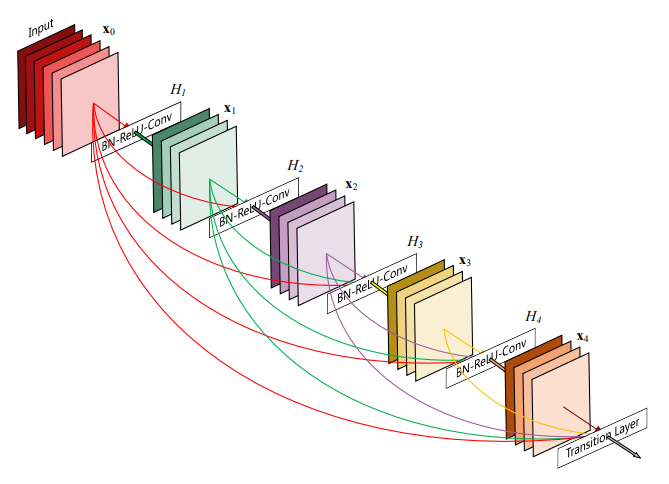
\includegraphics[width=0.8\linewidth]{images/densenet_hl}
	\caption{Kiến trúc DenseNet.}
	\label{fig:kien_truc_densenet}
\end{figure} 

Xét một hình ảnh $x_0$ duy nhất được truyền qua một mạng tích chập. Mạng bao gồm $L$ lớp, mỗi lớp thực hiện một phép biến đổi phi tuyến tính $H_l$(·), trong đó $l$ là chỉ mục các lớp. $H_l$(·) có thể là một hàm tổng hợp của các hoạt động như Batch Normalization (BN), lớp ReLU, lớp Pooling, hoặc lớp Convolution (Conv). chúng tôi biểu thị đầu ra của lớp thứ $l$ như là $x_l$.\\
{\bf Kết nối dày đặc - Dense connectivity}
Để cải thiện hơn nữa luồng thông tin giữa các lớp, chúng tôi đề xuất một mô hình kết nối khác: chúng tôi giới thiệu các kết nối trực tiếp từ bất kỳ lớp nào đến tất cả các lớp tiếp theo. Hình \ref{fig:kien_truc_densenet} minh họa bố trí kiến trúc của DenseNet. Dễ dàng nhìn thấy, lớp thứ $l$ nhận được các bản đồ đặc trưng của tất cả các lớp trước đó, $x_0, x_1, x_2, . . . , x_{l-1}),$ làm đầu vào:
\begin{equation}\label{eq:denseconnectivity}
	x_l = H_l([x_0, x_1, . . . , x_{l-1}])
\end{equation}
với $[x_0, x_1, . . . , x{l-1}]$ đề cập đến việc nối các trích chọn đặc trưng được tạo thành trong các lớp $0, 1, ..., {l-1}$. Do khả năng kết nối dày đặc của nó, chúng tôi gọi kiến trúc mạng này là Mạng kết nối dày đặc (DenseNet). Để dễ thực hiện, chúng tôi nối nhiều đầu vào của $H_l$(·) trong phương trình \ref{eq:denseconnectivity} thành một tensor duy nhất.\\
{\bf Hàm tổng hợp - Composite function}
chúng tôi định nghĩa $H_l$(·) là một hàm tổng hợp của ba hoạt động liên tiếp: Batch Normalization (BN), tiếp theo là một hàm tinh chỉnh các đơn vị tuyến tính (ReLU) và một tích chập 3 × 3 (Conv).\\
{\bf Tầng hợp nhất - Pooling layers}
